\documentclass[10pt]{article}

\usepackage{spheric}
%%%TITLE
\title{Hydrodynamics characteristics of land hinged Oscillating Wave Surge Converter with SPH method}
\date{}

%%AFFILIATIONS

\author[$\relax$]{D. H. Zhang}
\author[$\relax$]{Y. X. Shi$^\dagger$}
\author[$\relax$]{C. Huang}
\author[$\relax$]{Y. L. Si} 
\author[$\relax$]{B. Huang} 
\author[$\relax$]{W. Li}

\affil[$\relax$]{Ocean College, Zhejiang University, Zhou Shan, Zhejiang province, China}

\affil[$\relax$]{\href{mailto:yingxuan_shi@163.com}{yingxuan\_shi@163.com}}


%%DOCUMENT
\begin{document}

\maketitle

%\SelectedTopics{}

%%PLEASE PUT YOUR ABSTRACT HERE
\begin{abstract}
Wave energy is an abundant and dense form of renewable energy. One of the most promising Wave Energy Converters (WECs) is the bottom hinged Oscillating Wave Surge Converter (OWSC), such as Oyster (Figure \ref{fig:55-1}) which consists of a large buoyant flap hinged near the seabed. The flap oscillates back and forth under the action of the incident waves, and the kinetic energy of the flap is converted into electrical energy by pumping high pressure water ashore to drive a hydro-electric turbine. This design is good but when it is mounted on the sea bottom, several problems will appear, such as: difficulty in maintenance; corrosion by sea water; and oil leakage pollution \cite{do2015effects}. To avoid these problems, some researchers \cite{hansen2013discrete,zurkinden2014non} designed the land hinged OWSC (Figure \ref{fig:55-2}) whose hinged joints and hydraulic device can be placed above the water or on the coast. Although the land hinged OWSC is convenient in maintenance and avoids corrosion by sea water, it is still necessary to investigate its hydrodynamics characteristics which are directly related to wave power capturing efficiency. 
\begin{figure}[!htb]
\centering
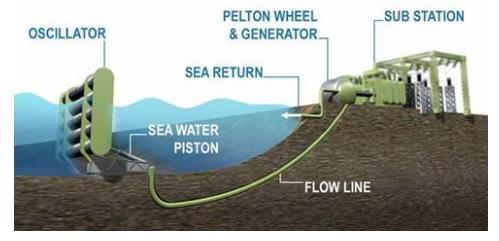
\includegraphics[width=0.72\textwidth]{55-1.png}
\caption{The sketch of Oyster}\label{fig:55-1}
\end{figure}
\begin{figure}[!htb]
\centering
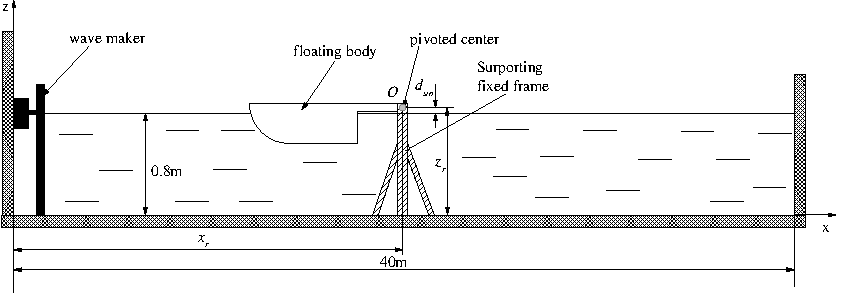
\includegraphics[width=0.75\textwidth]{55-2.pdf}
\caption{The sketch of single distributed absorbers}\label{fig:55-2}
\end{figure}

In this paper, Smoothed Particle Hydrodynamics (SPH) \cite{liu2010smoothed,monaghan2005smoothed} is used to the hydrodynamics characteristics of land hinged OWSC. The density diffusion model \cite{marrone2011delta} is used to remove the spurious high-frequency oscillations. Boundary force model \cite{hansen2013discrete} is used to avoid the penetration of fluid particles across the wall. The classic equations of rigid body dynamics are used to control the motions of OWSC. Stand waves, regular waves, and bottom hinged OWSC are simulated to validate accuracy of SPH method. The results of SPH are compared with the analytical solutions or reference results, and good agreements are achieved. These results demonstrate that SPH method presented in this paper can give acceptable results in the simulations of voilent waves.

Finally, the hydrodynamics characteristics of land hinged OWSC are investigated. Figure \ref{fig:55-2} shows the single land hinged OWSC model. The piston-type wavemaker is located on the left end of NWTs. A pivoted absorber is fixed and semi-immersed. Following harmonic wave loadings, absorber swings up and down around the rotation center $O$. As shown in Figure \ref{fig:55-3}(a) and Figure \ref{fig:55-3}(b), different absorber models are taken into consideration to study the effect of geometry profile on wave energy capturing efficiency. As shown in Figure \ref{fig:55-4}, two distributed absorbers with the fixed distances $D_b$ are simulated to investigate effect of $D_b$ on wave energy capturing efficiency. The results show that the active power of land hinged OWSC strongly depends on both the PTO damping coefficients and the wave periods. The optimized geometry profile may improve the efficiency of land hinged OWSC capturing wave energy. The distance of two distributed absorbers has important effect on wave energy capturing efficiency. 
\begin{figure}[!htb]
\centering
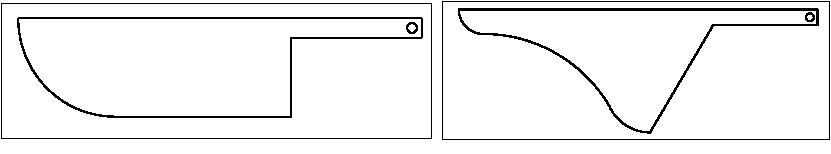
\includegraphics[width=0.75\textwidth]{55-3.pdf}
\caption{The geometry profile of pivoted absorber}\label{fig:55-3}
\end{figure}
\begin{figure}[!htb]
\centering
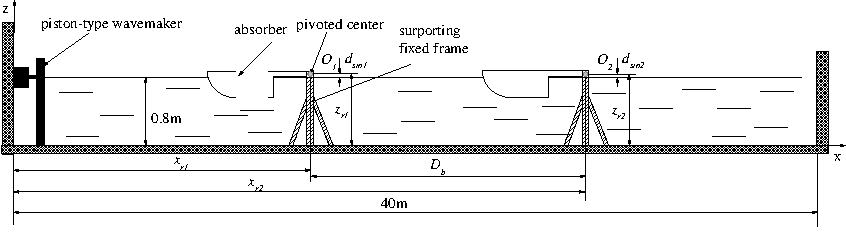
\includegraphics[width=0.75\textwidth]{55-4.pdf}
\caption{The sketch of two distributed absorbers}\label{fig:55-4}
\end{figure}

\end{abstract}


%%THE END OF ABSTRACT

\addbib

\end{document}
